\chapter{Blogging with WordPress}
WordPress has a blogging feature readily built-in. Enabling blogging on the website is very simple and require only a few steps. This chapter will explain how to create a new blog spot, publishing it, and adding a menu link to the blog post entries.

\section*{Step 1: Login into admin side}
First, login into admin side of the website by accessing the following URL:
\begin{lstlisting}
http://<base-url>/wp-admin

http://web.smarthome.hs-furtwangen.de/wp-admin
\end{lstlisting}

In case the base URL has been changed, just add the relative URL \texttt{/wp-admin} to access the admin side of the website. The admin side of any WordPress powered website is accessed through this relative path.

\section*{Step 2: Username and password}
As of the point of writing, there is only username has been created. Login into admin side using the following credentials:
\begin{itemize*}
\item Username: ashiqmoh
\item Password: oSm0cCCAguIMsalrZd(\#2i5(
\end{itemize*}

\section*{Optional Step: Creating a new user}
In the future, if required, additional users can be added to website by accessing the \scalerel*{
\includegraphics{blogging/users-menu.png}}{B} menu and subsequently \scalerel*{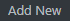
\includegraphics{blogging/add-new-user-submenu.png}}{B} item on the left navigation. This will show a page with fields such as \emph{Username}, \emph{Email}, \emph{First Name}, \emph{Last Name}, and \emph{Website} to be entered.

Only the \emph{Username} and \emph{Email} fields are mandatory. The password will be auto-generated and sent to the email address of the new user automatically. But WordPress also allow the password to be seen and be given manually by clicking the \scalerel*{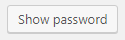
\includegraphics{blogging/show-password.png}}{B} button while creating a new user.

Another important thing while creating a new user is to assign the appropriate \emph{Role}. There are five types of role, which are:
\begin{itemize*}
\item Subscriber
\item Contributor
\item Author
\item Editor
\item Administrator
\end{itemize*}

For the user that requires the permission to do blogging should be assigned with the role of \emph{Editor} or \emph{Author}. The difference \cite{wp-user-roles} between these two roles are as follow:
\begin{description}
\item[Editor] is somebody who can publish and manage posts including the posts of other users.
\item[Author] is somebody who can publish and manage their own posts only.
\end{description}

\section*{Step 3: Creating a new blog entry}
The blog section can be accessed by clicking the \scalerel*{
\includegraphics{blogging/posts-menu.png}}{B} menu on the left menu navigation. When this menu has been clicked, a listing of all the blog entries (see Figure~\ref{fig:blog-entries}) will be shown. As at the point of writing, there is only one blog entry in the website. The title of the blog is "First blog entry" with the content "Hello, world!".

\begin{figure}[ht]
\caption{Blog entries}
\label{fig:blog-entries}
\centering
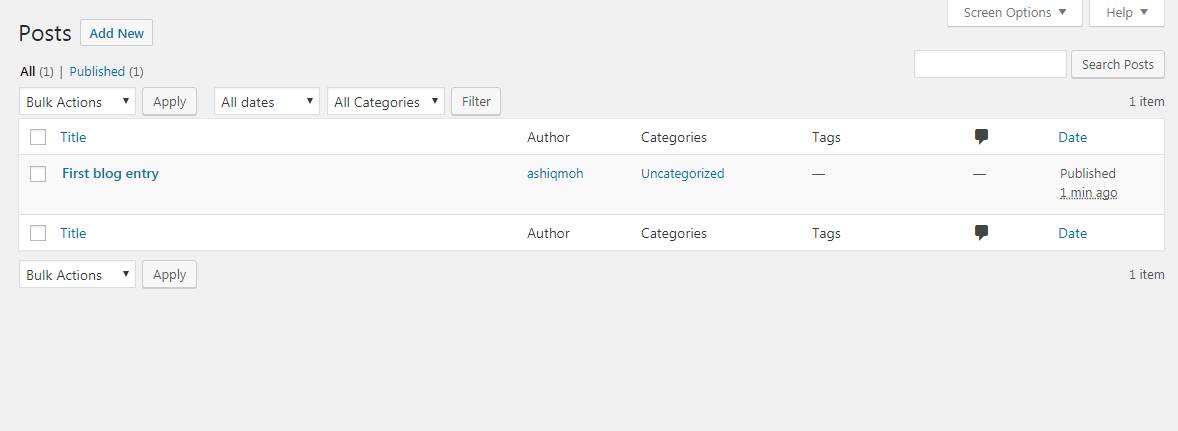
\includegraphics[width=.65\linewidth,keepaspectratio]{blogging/blog-entries.png}
\end{figure}

In order to create a new blog entry, click on the \scalerel*{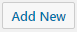
\includegraphics{blogging/add-new-post.png}}{B} button, which can be found on the top left of the blog post entries. When this button has been clicked, a new page will appear as shown in Figure~\ref{fig:new-post-entry}.

\begin{figure}[ht]
\caption{New blog (post) entry}
\label{fig:new-post-entry}
\centering
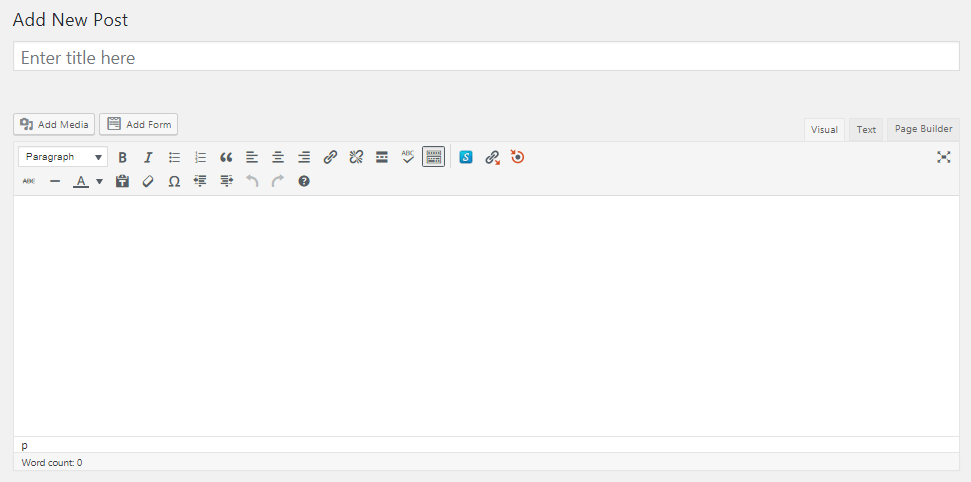
\includegraphics[width=.65\linewidth,keepaspectratio]{blogging/new-post-entry.png}
\end{figure}

Here, the title of the blog post has to be given in the text field with the placeholder \emph{Enter title here} (refer Figure~\ref{fig:enter-title-here}). Next, make sure that the text editor is in the \emph{Visual} mode (refer Figure~\ref{fig:editor-visual-mode}). The visual mode provides a semi \ac{wysiwyg} content editor, which enable an easy way to create, edit and format the blog post contents in view similar to that of a word processor \cite{wordpress-editor}.

\begin{figure}[ht]
\caption{Text field for blog post title}
\label{fig:enter-title-here}
\centering
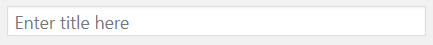
\includegraphics[width=.5\linewidth,keepaspectratio]{blogging/enter-title-here.png}
\end{figure}

\begin{figure}[ht]
\caption{Text editor setting to 'Visual' mode}
\label{fig:editor-visual-mode}
\centering
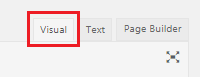
\includegraphics[width=.4\linewidth,keepaspectratio]{blogging/editor-visual-mode.png}
\end{figure}

\section*{Step 5: Publishing the blog post}
After finish editing the blog post content, the post can be published by clicking the  \scalerel*{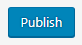
\includegraphics{blogging/publish.png}}{B} button as shown in the Figure~\ref{fig:publish-post-box}. Other than that, WordPress also offers the options to save the blog post without publishing it into the website. This can be done clicking the 'Save Draft' button.

\begin{figure}[ht]
\caption{Publishing blog post}
\label{fig:publish-post-box}
\centering
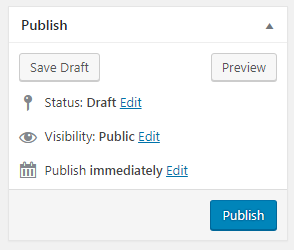
\includegraphics[width=.4\linewidth,keepaspectratio]{blogging/publish-post-box.png}
\end{figure}

\section*{Step 6: Previewing the blog post entry}
The edited blog post can be viewed or previewed by clicking the \scalerel*{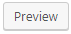
\includegraphics{blogging/preview.png}}{B} button before publishing it. If the blog post has been published, the button will change into \scalerel*{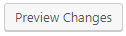
\includegraphics{blogging/preview-changes.png}}{B}. This button also has the same functionality as the preview button. Another way of previewing the blog entry is by clicking the permalink that appears below the 'Title' text field as shown in Figure~\ref{fig:permalink-blog-post}.

\begin{figure}[ht]
\caption{Permalink below 'Title' text field}
\label{fig:permalink-blog-post}
\centering
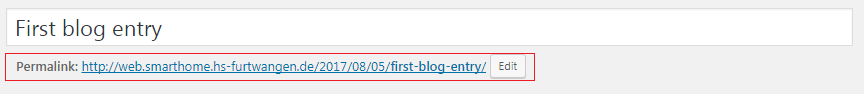
\includegraphics[width=.7\linewidth,keepaspectratio]{blogging/permalink.png}
\end{figure}

Note: The permalink only will appear when the user start editing the new post. It won't appear at the beginning.

\section*{Step 7: Adding menu for blog entry}
When blogging has been started, a menu has to be added to the main navigation menu (refer Figure~\ref{fig:main-menu}) that at appears at the header part of the website. Currently, there is no menu link that links the website to the blog entries. This section will explain how to add one.

\begin{figure}[ht]
\caption{Main navigation menu}
\label{fig:main-menu}
\centering

\includegraphics[width=.8\linewidth,keepaspectratio]{blogging/main-menu.png}
\end{figure}

From the left navigation panel on the admin side, access the \scalerel*{
\includegraphics{blogging/appearance-menu.png}}{B} menu and followed by  \scalerel*{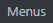
\includegraphics{blogging/menus-menu.png}}{B} submenu. A screen as shown in the Figure~\ref{fig:menu-screen} will appear. First, expand the \emph{Pages} accordion menu has been highlighted in the figure.

\begin{figure}[ht]
\caption{Menu screen}
\label{fig:menu-screen}
\centering
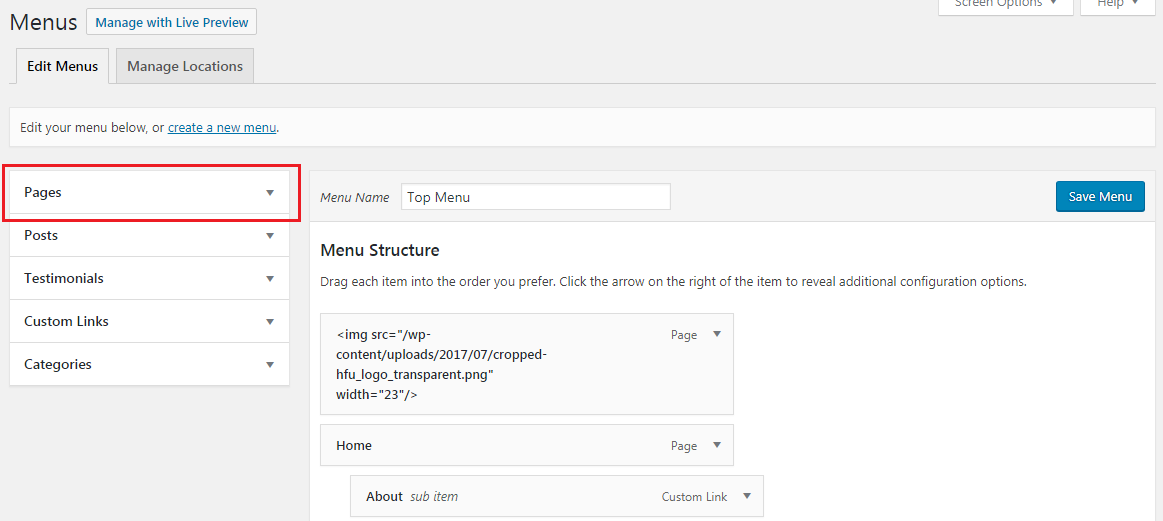
\includegraphics[width=.8\linewidth,keepaspectratio]{blogging/menu-screen.png}
\end{figure}

Then, check the checkbox \emph{Blog} and click the \scalerel*{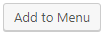
\includegraphics{blogging/add-to-menu.png}}{B} button. This will add a link linking blog post entry to the main navigation menu as shown in the Figure~\ref{fig:main-menu}.

\begin{figure}[ht]
\caption{Adding a menu to link blog post}
\label{fig:checking-blog-checkbox}
\centering
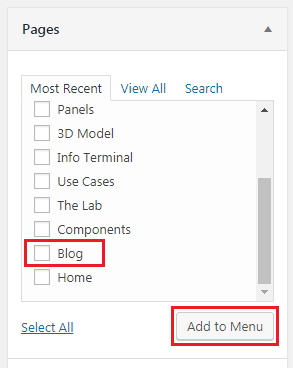
\includegraphics[width=.4\linewidth,keepaspectratio]{blogging/checking-blog-checkbox.png}
\end{figure}

After adding the \emph{Blog} menu by clicking the \scalerel*{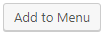
\includegraphics{blogging/add-to-menu.png}}{B}, the \emph{Blog} menu will appear under the \emph{Menu Structure} column on the right (refer Figure~\ref{fig:menu-structure}). Here, the position of the link can re-ordered by dragging and dropping, as the new menu will be added as a last menu item by default.

\begin{figure}[ht]
\caption{Menu structure column}
\label{fig:menu-structure}
\centering
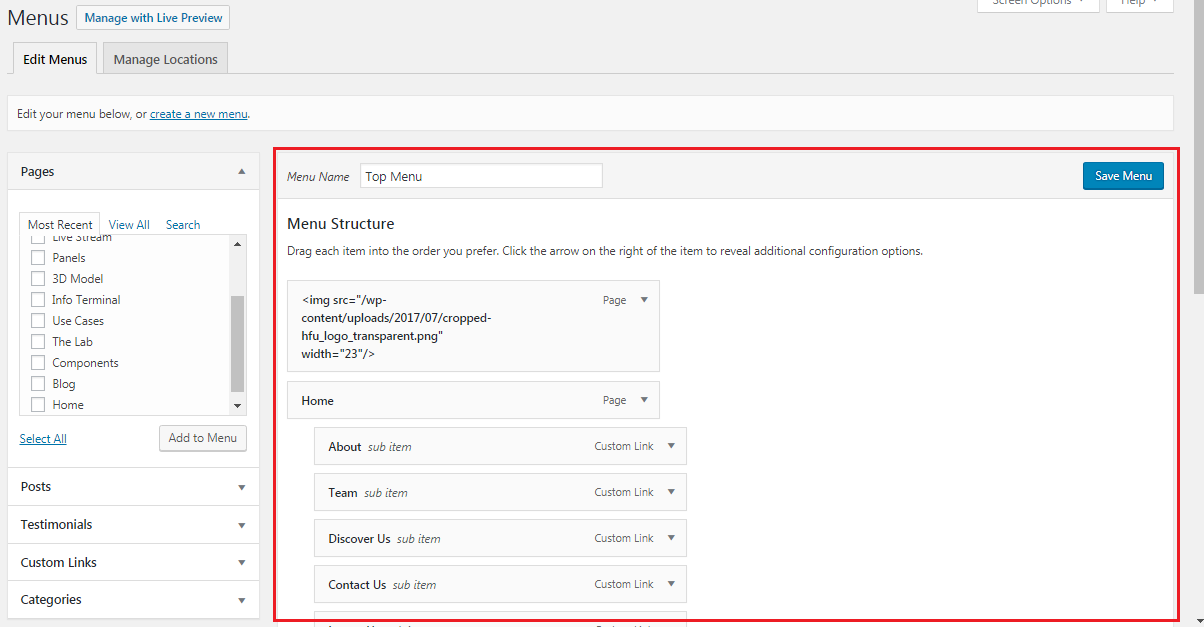
\includegraphics[width=.8\linewidth,keepaspectratio]{blogging/menu-structure.png}
\end{figure}

After reordering the \emph{Blog} menu to the desired position, save the added menu by clicking the \scalerel*{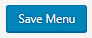
\includegraphics{blogging/save-menu-button.png}}{B} button on the top right of \emph{Menu Structure} column on the web page.
